\chapter{Introducción}
Los sistemas de adquisición de datos juegan un papel importante en una amplia variedad de campos, debido a que la precisión y el control de datos son esenciales para el avance tecnológico.

Estos sistemas permiten capturar, procesar y analizar señales provenientes de sensores y dispositivos, siendo indispensables en áreas como la automatización industrial, la investigación científica y el control de procesos. Ya sea para monitorear variables como temperatura, presión o voltaje, o incluso para obtener imágenes detalladas de detectores infrarrojos en cámaras térmicas y dispositivos de visión nocturna, los sistemas de adquisición de datos se destacan por su capacidad de registrar información de forma precisa y eficiente. Su versatilidad los convierte en herramientas clave para el desarrollo de tecnologías innovadoras en diversas áreas.


Desarrollar un sistema de adquisición de datos para obtener imágenes térmicas es esencial debido a las múltiples aplicaciones de las imágenes infrarrojas, que van desde la seguridad y vigilancia en hogares \cite{Yii2023}, hasta el diagnóstico médico para determinar diabetes \cite{LeneroBardallo2022}, detección de gestos \cite{LeBa2019} y el monitoreo ambiental. Los detectores infrarrojos juegan un papel crucial en estos sistemas, ya que permiten capturar radiación térmica que no es visible al ojo humano, proporcionando información valiosa sobre la distribución de temperatura en una escena. Esta capacidad es fundamental en situaciones como la detección de fallas en equipos eléctricos, la monitorización de la temperatura corporal, o la identificación de focos de calor en incendios forestales. 


Debido a la importancia de los sistemas de adquisición de datos en aplicaciones que utilizan detectores infrarrojos, es fundamental comprender el comportamiento de estos detectores. Conocer cómo responden a diferentes condiciones de luz y temperatura permite diseñar sistemas más eficientes y precisos para capturar imágenes térmicas.
    
    \section{Radiación Electromagnética}
    La radiación electromagnética es la emisión y transmisión de energía en forma de ondas electromagnéticas. El espectro electromagnético es una representación de los diversos tipos de radiación existentes, en él se definen los intervalos de longitudes de onda o frecuencia que cada una de ellas abarca \cite{Chang}.
            \begin{figure}[hbtp]
                \centering
                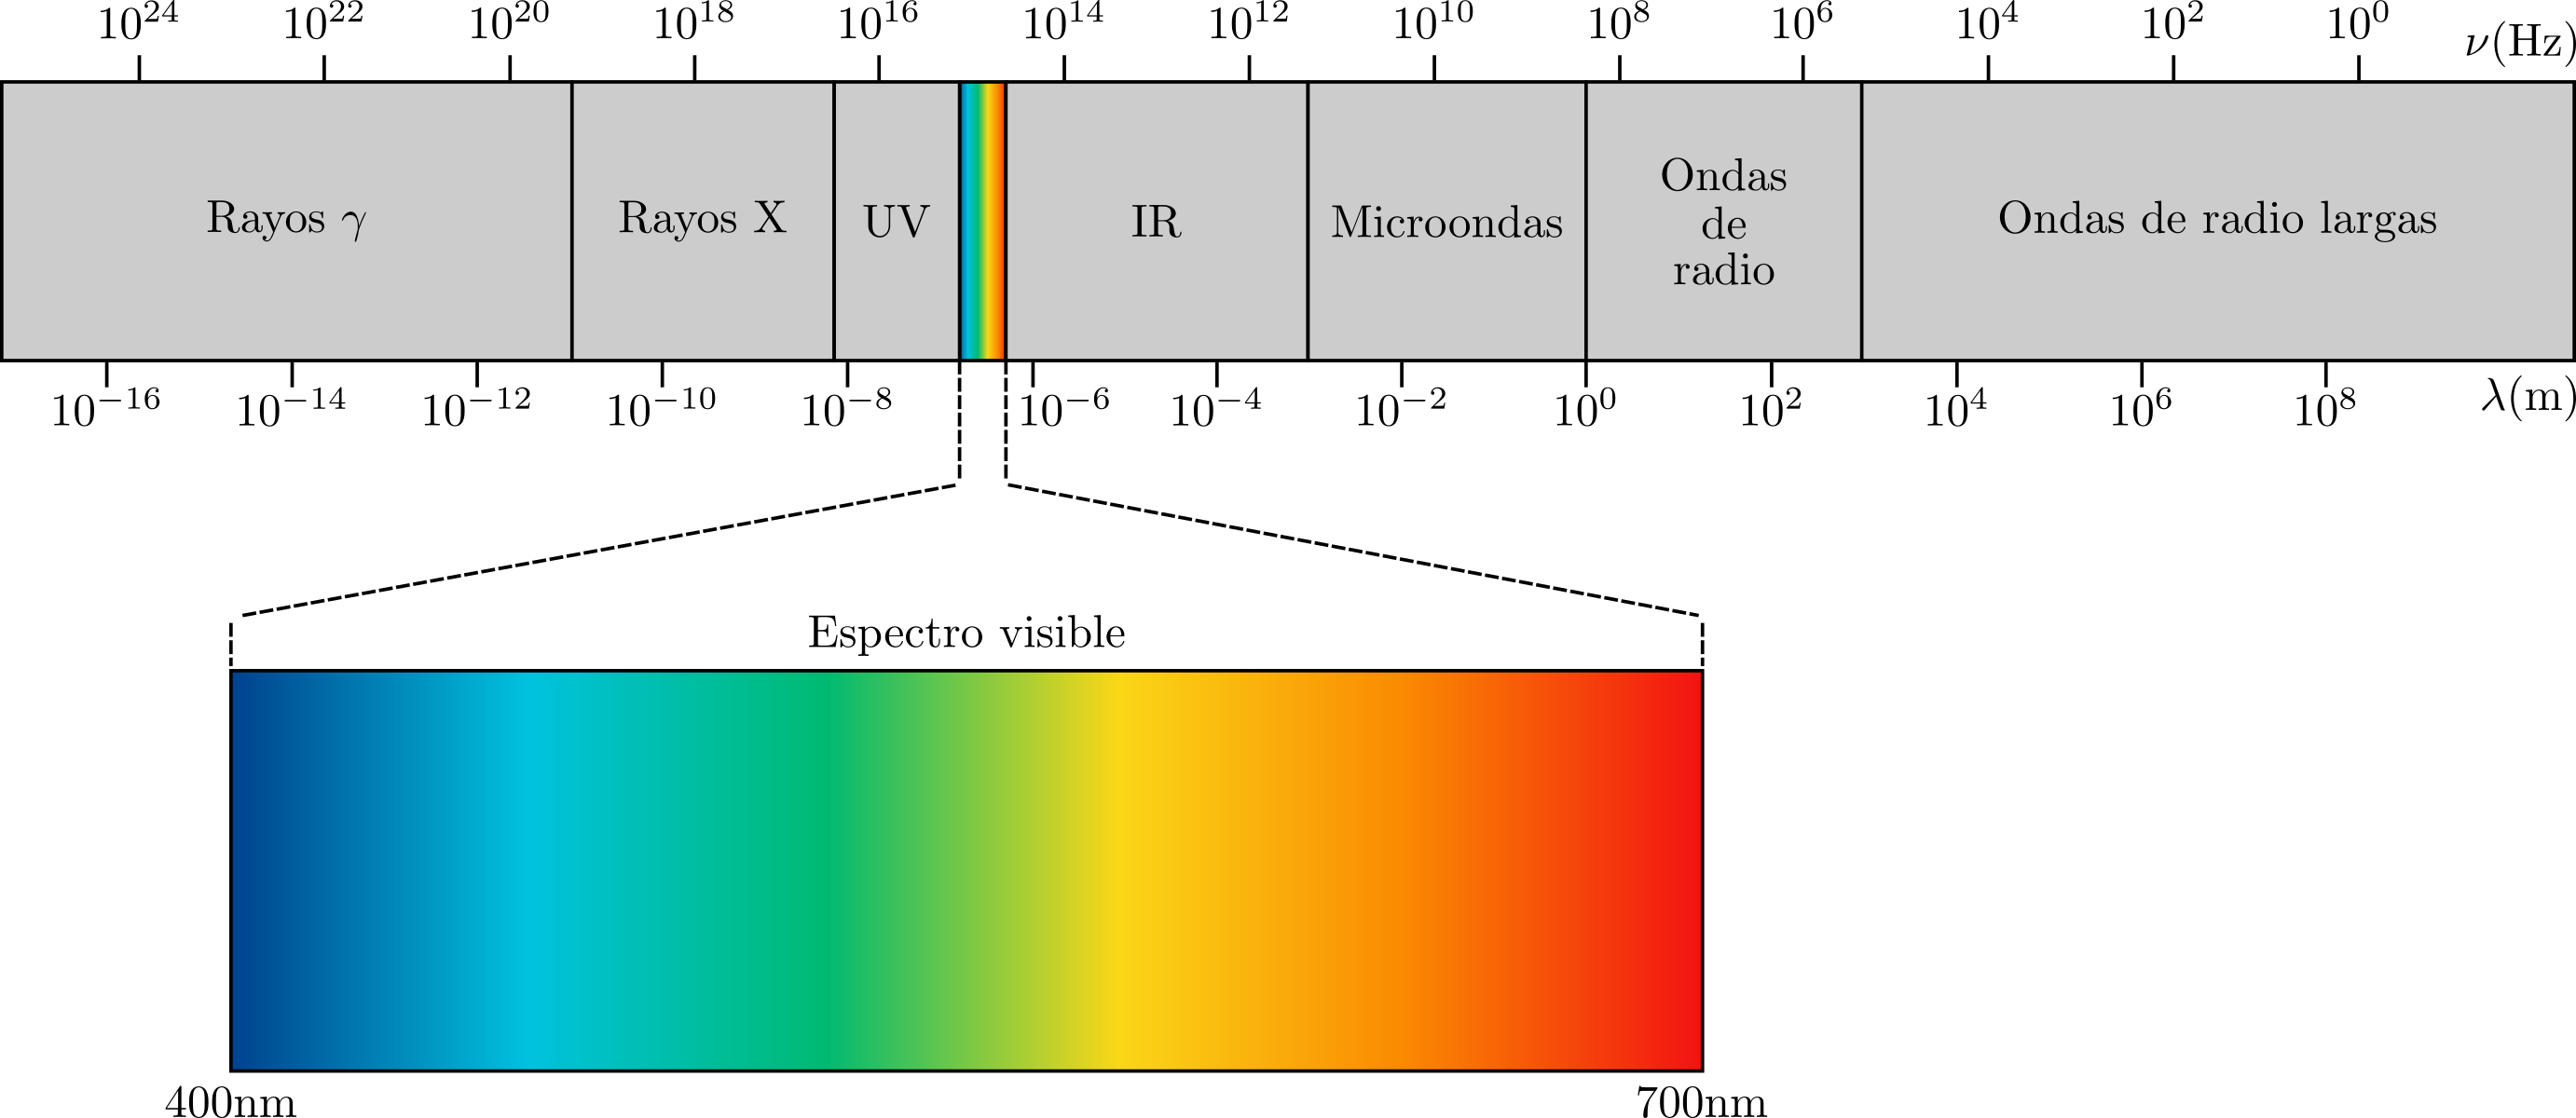
\includegraphics[width=0.8\textwidth]{espectro}
                \caption{Espectro electromagnético.}
                \label{fig:espectro}
            \end{figure}    
    
    Estas radiaciones obedecen las mismas leyes, la diferencia entre ellas radica en su longitud de onda o frecuencia, así como en la manera en que interactúan con los materiales ópticos, incluída la atmósfera \cite{Vincent}.
    
    Todos los cuerpos emiten radiación e.m  y debido al movimiento de sus átomos y moléculas se genera una temperatura en ellos. Los cuerpos con una temperatura mayor a 0K emiten radiación térmica por medio de ondas e.m. La radiación térmica es la radiación que emite un cuerpo por su temperatura \cite{Hollands}.
    
    La capacidad que tiene un cuerpo para emitir radiación está fuertemente relacionada con su capacidad de absorberla \cite{Beiser}.
    
    Una superficie ideal que absorbe toda la radiación que incide sobre él se denomina \textit{cuerpo negro} y el espectro de radiación que emite se llama \textit{radiación de cuerpo negro} \cite{Sears}.
    
    A pesar de que en la naturaleza no existe un objeto físico que pueda absorber toda la radiación incidente \cite{FUV3}, este puede representarse como un objeto hueco con una pequeña apertura donde cualquier radiación que incida en ella ingresa a la cavidad donde queda atrapada hasta que es absorbida \cite{Beiser}, \cite{FUV3}. En equilibrio térmico la radiación emitida por el cuerpo será exactamente igual a la absorbida.
    
    El cuerpo negro fue creado como una herramienta auxiliar para entender como los objetos emiten y absorben radiación.
    Hacia finales del siglo XIX la radiación de cuerpo negro ya había sido estudiada y dos leyes importantes sintetizaron los descubrimientos experimentales sobre este tema: La \textit{Ley de Stefan-Boltzmann} y la \textit{Ley de desplazamiento de Wien} \cite{FUV3}.
    
    La \textit{Ley de Stefan-Boltzmann} plantea que la intensidad de la radiación emitida por un cuerpo negro depende de su temperatura. La intensidad es proporcional a la cuarta potencia de la temperatura absoluta del cuerpo:
    
    \begin{equation}
        I = \sigma T^{4}
        \label{eq:Stefan-Boltzmann}
    \end{equation}
    donde:
    
    $T$ es la temperatura del cuerpo negro en K.
    
    $\sigma$ es la constante de Stefan-Boltzmann, $\sigma = 5.670\times10^{-8}\ W/m^{2}K^{4}$
    
    La intensidad de la radiación no se distribuye uniformemente a lo largo de todas las longitudes de onda. En cambio, su distribución puede medirse y describirse utilizando la intensidad por intervalo de longitud de onda, $I(\lambda)d\lambda$.
            \begin{figure}[hbtp]
                \centering
                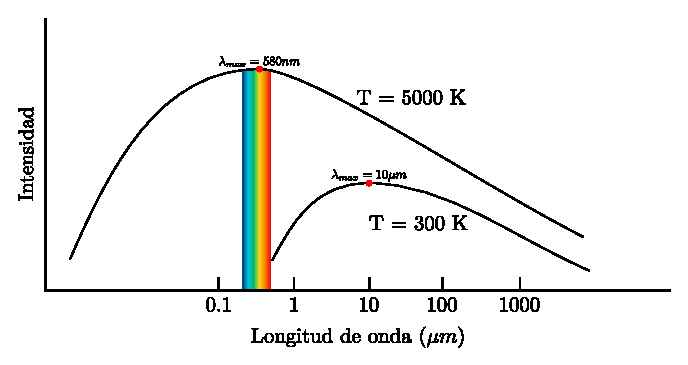
\includegraphics[width=0.8\textwidth]{intensidad_bb}
                \caption{Emitancia espectral de un cuerpo negro.}
                \label{fig:intensidad_bb}
            \end{figure}    
    \newpage
    La Figura \ref{fig:intensidad_bb} muestra las intensidades registradas a dos temperaturas diferentes. En cada caso hay una longitud de onda específica $\lambda_{m}$ en la que la intensidad de la radiación emitida es máxima.
    
    La \textit{Ley de desplazamiento de Wien} indica que cuando la temperatura de un cuerpo negro aumenta, la longitud de onda en la que se emite la radiación máxima se desplaza hacia valores más cortos:
    
    \begin{equation}
        \lambda_{m} = \frac{2.90\times10^{-3}\ mK}{T}
        \label{eq:Wien}
    \end{equation}   
    donde:
    
    $\lambda_{m}$ es la longitud de onda en la que un cuerpo negro emite la mayor cantidad de radiación a una determinada temperatura \cite{Sears},\cite{FUV3}.
    
    De las leyes anteriores y la Figura \ref{fig:intensidad_bb} se puede deducir que la radiación UV, los rayos X y Gamma, son radiaciones más cálidas (radiaciones de alta energía), mientras que la radiación infrarroja está asociada a fenómenos con temperaturas cercanas a la temperatura ambiente \cite{Chang}, \cite{BlancoMDA}.     
    
    \section{Radiación Infrarroja} 
    La radiación infrarroja es un tipo de radiación electromagnética que cuenta con longitudes de onda mayores que las del rango visible. Se encuentra en el rango de 0.77$\mu m$ - 1$mm$ \cite{BlancoMDA}, y a su vez se divide en varias regiones las cuales se muestran en la Tabla \ref{tab:Div_IR} \cite{Rogalski}.
    
            \begin{table}[htbp]
                \caption{División de la radiación infrarroja.}
                \begin{center}
                    \resizebox{0.8\linewidth}{!}{ 
                    \begin{NiceTabular}{|l|c| }
                        \CodeBefore
                        \Body
                        \hline
                        \textbf{Region}  & \textbf{Rango de frecuencia ($\mu m$)}\\
                        \hline
                        Near infrared (NIR)   & 0.78 - 1\\
                        Short wavelength IR (SWIR)   & 1 - 3\\
                        Medium wavelength IR (MWIR) & 3 - 6\\
                        Long wavelength IR (LWIR)  & 6 - 15\\
                        Very long wavelength IR (VLWIR) & 15 - 30\\
                        Far infrared (FIR)  & 30 - 100\\
                        Submillimeter (SubMM) & 100 - 1000\\
                        \hline
                    \end{NiceTabular}
                    }
                \label{tab:Div_IR}
                \end{center}
            \end{table}
            
            \newpage
            
Algunas de las aplicaciones de la radiación infrarroja son:
			\begin{itemize}
				\item \textbf{Visión nocturna}: Las cámaras de visión nocturna trabajan en el espectro infrarrojo para permitir la visión en la oscuridad, estas capturan la radiación térmica emitida por objetos y seres vivos.
				\item \textbf{Medicina}: Es utilizada para hallar cáncer y diabetes en el cuerpo humano.
				\item \textbf{Industria}: Inspección del estado de equipos eléctricos y mecánicos.
				\item \textbf{Conservación de energía}: Con escáneres IR se detectan pérdidas y fugas de calor en casas o industrias.
				\item \textbf{Ambientales}: Medición de la concentración de diversos gases contaminantes en la atmósfera.
				\item \textbf{Agricultura}: Monitoreo del estado de los cultivos y la salud de las plantas, la humedad del suelo y la presencia de plagas o enfermedades.
				\item \textbf{Astronomía}: Los telescopios infrarrojos permiten estudiar regiones del espacio donde se están formando estrellas.
				\item \textbf{Espectroscopía}: Usada en química y biología para identificar y analizar estructuras moleculares de sustancias.		
			\end{itemize}
\cite{Rogalski}, \cite{BlancoMDA}.

La mayoría de las aplicaciones en detección de radiación infrarroja requieren que esta se transmita a través del aire \cite{Jimenez}. La atmósfera terrestre se compone de ozono ($O_{3}$), dióxido de carbono ($CO_{2}$) y vapor de agua ($H_{2}O$). Estas moléculas bloquean algunas regiones del espectro infrarrojo, impidiendo la transmisión de la radiación IR a la atmósfera. Las longitudes de onda que no son afectadas por estas moléculas reciben el nombre de ventanas atmosféricas \cite{Rogalski}, \cite{Motilal}. En la Figura \ref{fig:atmos_window} podemos observarlas.

            \begin{figure}[hbtp]
                \centering
                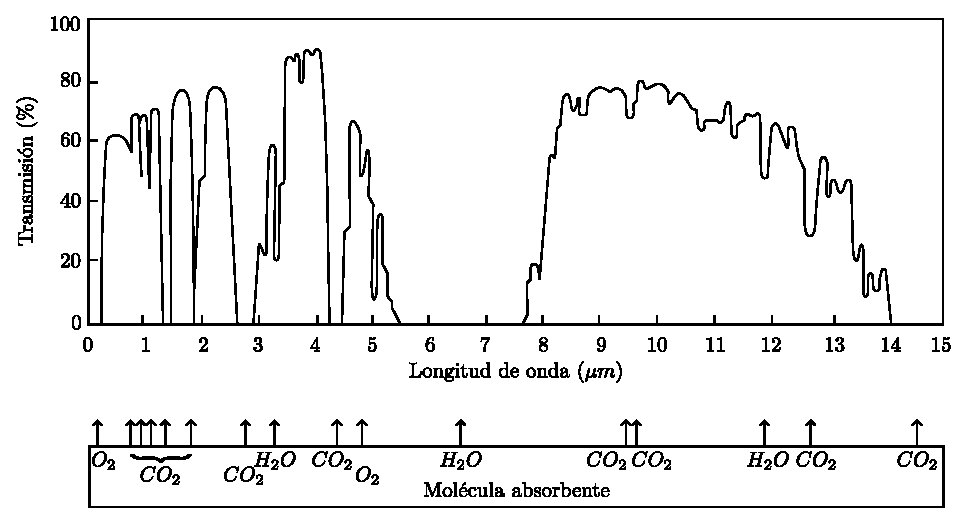
\includegraphics[width=0.8\textwidth]{atmos_window}
                \caption{Transmisión de la atmósfera.}
                \label{fig:atmos_window}
            \end{figure}



Despejando la temperatura de la ecuación \ref{eq:Wien} \cite{BlancoMDA}:
    \begin{equation}
        T_{max} = \frac{2.90\times10^{-3}\ mK}{8\mu m} = 362.5K
        \label{eq:tempmax}
    \end{equation}

    \begin{equation}
        T_{min} = \frac{2.90\times10^{-3}\ mK}{14\mu m} = 207.14K
        \label{eq:tempmin}
    \end{equation}

podemos deducir que los detectores infrarrojos que operan en la ventana de 8 - 14 $\mu m$ tienen mayor sensibilidad a la temperatura ambiente \cite{Rogalski}.

El material de fabricación y longitud de onda de operación de los detectores infrarrojos cambian de acuerdo a la aplicación en la que se desee trabajar \cite{Rogalski}.					           
     
    
    \section{Detectores Infrarrojos}
    
    Un detector infrarrojo es un dispositivo capaz de absorber parte de la energía infrarroja radiada hacia él, provocando una variación en alguna de sus propiedades eléctricas \cite{BlancoMDA}. Podemos pensar en un detector infrarrojo como un transductor, el cual convierte un tipo de señal en otra; el detector infrarrojo convierte la radiación infrarroja incidente en una señal eléctrica \cite{Vincent}.
    
    Dependiendo de la aplicación, el rango del espectro electromagnético y la temperatura en los que se desee trabajar, se debe diseñar o utilizar un detector específico que cumpla con los requerimientos, ya que cada aplicación requiere características diferentes a las demás \cite{Rogalski},\cite{BlancoMDA}.
    
    Los detectores infrarrojos se pueden clasificar en dos categorías: \textit{Detectores de fotones} y \textit{detectores térmicos}.
    
		\subsection{Detectores de fotones}
		En los detectores de fotones, la formación de pares electrón-hueco es consecuencia de la detección de radiación absorbida \cite{BlancoMDA}. En estos dispositivos, el fotón que incide sobre la superficie del material puede ser absorbido, lo que resulta en la remoción de un electrón desde la banda de valencia o desde un estado localizado dentro de la banda prohibida hasta la banda de conducción.

Generalmente, los detectores de fotones que operan a longitudes de onda de aproximadamente 3$\mu m$ requieren de un sistema de enfriamiento. Esto es necesario para prevenir la generación térmica de portadores de carga, la cual es su principal desventaja, ya que aumenta su costo y complejidad de operación. No obstante, su resolución y desempeño son bastante buenos \cite{Vincent},\cite{BlancoMDA}. 
		   
		\subsection{Detectores térmicos}
		El funcionamiento de los detectores térmicos se basa en la generación de una salida eléctrica medible como resistencia o diferencia de potencial debido al cambio de temperatura del material causado por la radiación incidente.
Estos detectores pueden funcionar a temperatura ambiente, son económicos, compactos, de bajo consumo energético y tienen una larga vida útil, pero su capacidad de detección es baja \cite{Rogalski},\cite{BlancoMDA}.
Algunos de los principales detectores térmicos infrarrojos son explicados a continuación.
		
		\subsubsection{Celda de Golay}
		La celda de Golay es un detector térmico principalmente utilizado en espectroscopía infrarroja, la celda consiste en una cámara herméticamente cerrada llena de gas y un espejo flexible. A medida que la radiación infrarroja incide, el gas se calienta y se expande, provocando que el espejo flexible se mueva. El movimiento del espejo desvía un haz de luz que incide sobre otro detector generando un cambio en su irradiancia, después esa señal es procesada \cite{Vincent},\cite{BlancoMDA}.
		\subsubsection{Bolómetros y Microbolómetros}
		Los bolómetros y microbolómetros son dispositivos que detectan la radiación infrarroja mediante el cambio en la resistencia eléctrica de un material al variar su temperatura. Conforme la resistencia absorbe calor, su temperatura aumenta y su resistencia se modifica.
Este tipo de sensores deben polarizarse con corriente o voltaje para que puedan funcionar.
Si son polarizados con corriente, el cambio de la resistencia se puede detectar y medir como un cambio de tensión, pero si se polariza con voltaje entonces se detectará como un cambio de corriente \cite{Rogalski},\cite{Vincent}.
		\subsubsection{Termopares y Termopilas}
		Los termopares y las termopilas están formados por la unión de dos conductores diferentes unidos por un extremo. Cuando la temperatura aumenta en esa unión, se genera una diferencia de potencial. Al conectar en serie varias uniones de conductores, se produce una tensión más elevada y, por lo tanto, medible \cite{Rogalski},\cite{Vincent}.
		
		\subsubsection{Detectores piroeléctricos y ferroeléctricos}
		Estos detectores pueden visualizarse como un capacitor con dos electrodos metálicos colocados perpendicularmente. Cuando un detector piroeléctrico absorbe radiación, su temperatura cambia, lo que genera una carga en el capacitor y una corriente que depende del cambio de temperatura. Si la temperatura permanece constante, la corriente será nula.

Los detectores ferroeléctricos operan bajo el mismo principio que los piroeléctricos, pero con la diferencia de que el efecto se produce mediante un campo eléctrico \cite{Rogalski}, \cite{BlancoMDA}.

		
En los últimos años, ha habido un creciente interés en el uso de microbolómetros para generar imágenes infrarrojas, superando a otros tipos de sensores en diversas aplicaciones, incluyendo el área médica. Este interés se debe, en parte, a las dimensiones reducidas de los microbolómetros, que pueden ser menores a $12 \mu m$, lo que permite una mayor densidad de píxeles en el sensor. Además, mientras que la resolución de algunos sensores infrarrojos está limitada a un arreglo de $120 \times 84$ píxeles, los microbolómetros pueden alcanzar resoluciones mucho más altas, como $1280 \times 1024$ o más, obteniendo imágenes más detalladas y nítidas. En el ámbito médico, los microbolómetros se han utilizado para detectar la temperatura corporal \cite{Svantner2022} y, de manera innovadora, en el diagnóstico de la diabetes, capturando imágenes térmicas de la lengua \cite{WziatekKuczmik2024} o del pie \cite{Rocha2022} para identificar variaciones térmicas que pueden indicar problemas de salud. Estas capacidades hacen de los microbolómetros una opción preferida en tecnologías de imágenes térmicas de alta precisión.
		 					          
		
    \section{Objetivos}
	
		\subsection{Objetivo general}
			\begin{itemize}
				\item Diseño de un sistema de adquisición de datos basado en FPGA para la medición de una matriz de pixeles de un microbolómetro.
			\end{itemize}
		
		\subsection{Objetivos específicos}
			\begin{itemize}
                \item Obtención de especificaciones para el sistema de adquisición de datos.
                \item Selección de ADC y DAC y protocolo de comunicación a partir de las especificaciones.
                \item Diseño de un firmware en el lenguaje de descripción de hardware (HDL) Verilog para el protocolo de comunicación SPI reconfigurable y robusto.
                \item Implementación de protocolo SPI para control de un ADC y un DAC de 12 bits.
                \item Pruebas experimentales y de estrés para verificación de robustes del diseño y mejora.
                \item Adquisición de los datos utilizando una terminal de usuario basada en UART.
			\end{itemize}
